% !TEX root = ../main.tex
\section{Leptospirosis: the stretch goal}
\label{sec:lepto}

The proposal assumed that no open subnational leptospirosis series exists. Project CCHAIN on HDX has weekly counts from the Philippine Integrated Disease Surveillance and Response (PIDSR) system for \leptoNCities{} cities, and a national weekly series of notifiable diseases is published on Mendeley Data. Both are analysed as \textbf{retrospective associations}, not forecasts: negative-binomial models of weekly cases on CHIRPS rain 0 to \leptoMaxLag{} weeks earlier, with seasonal terms, year and city effects and a COVID-19 term. Figure~\ref{fig:lepto} shows the incidence rate ratios (IRR) by lag.

\begin{figure}[htbp]
\centering
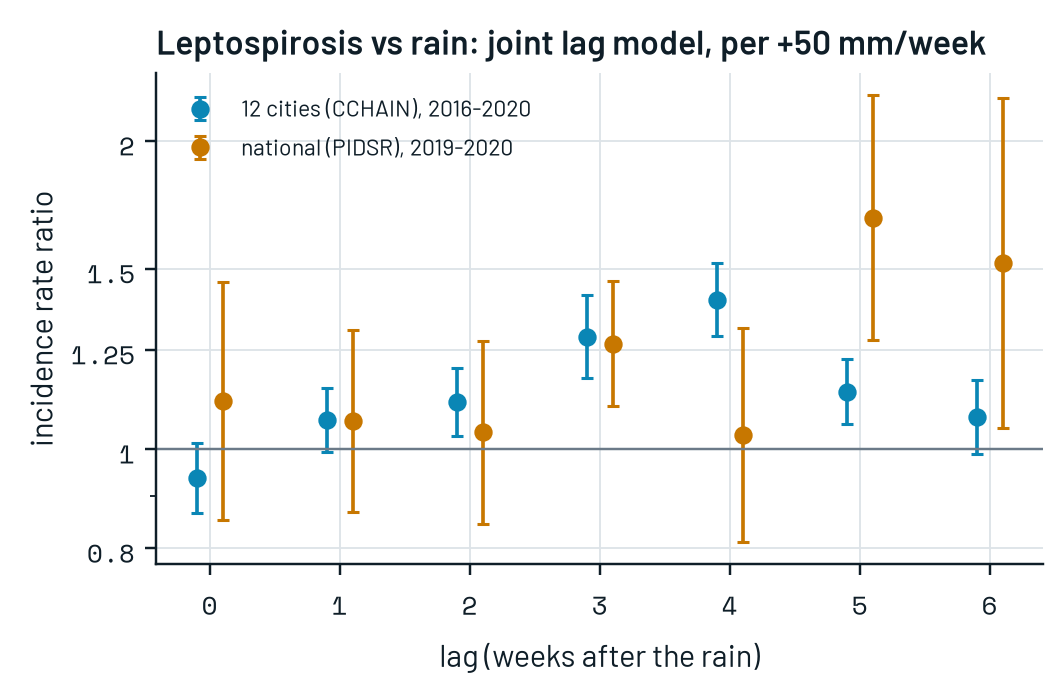
\includegraphics[width=0.72\linewidth]{f17_lepto}
\caption{Joint distributed-lag incidence rate ratios (95\% confidence intervals) per +\leptoRainPer{}~mm/week of rain, for the cities and the national series.}
\label{fig:lepto}
\end{figure}

\begin{itemize}
\item \textbf{Cities (\cityObs{} city-weeks, \cityCases{} cases, 2016--2020): the headline.} Rain is followed by leptospirosis \citySigRange{} weeks later; the joint peak is at lag \cityPeakLag{}, IRR \cityPeakCI{} per +\leptoRainPer{}~mm/week, and the cumulative IRR over lags 0 to \leptoMaxLag{} is \cityCumCI{}. A heavy-rain week (at or above the city's \leptoHeavyPctl{} percentile) peaks at lag \heavyPeakLag{}: \heavyPeakCI{}. That is a week or two later than the peak of \litLeptoPeak{} found in an earlier Philippine study \parencite{matsushita2018}; the CCHAIN week label is uncertain by about a week.
\item \textbf{National (\natObs{} weeks, 2019--2020): consistent, weaker.} The joint peak is at lag \natPeakLag{}, \natPeakCI{}; the cumulative IRR is \natCumCI{}. With 2019 alone the cumulative effect is \natNineteenCumCI{}: much of the national signal comes from 2020 (the December surge after Rolly and Ulysses, under COVID-19 reporting).
\item \textbf{Typhoons: mixed.} After Rolly and Ulysses (2020), cities inside the gale swath had \didRUPost{} times the outside cities' ratio of observed to expected cases in weeks 1 to 4 (pre-landfall placebo \didRUPre{}). For Ompong and Tisoy the ratio is \didOTPost{} but the placebo fails (\didOTPre{}): weeks of monsoon rain had already raised cases before Ompong. Four storms and \leptoNCities{} cities support no general storm effect.
\item \textbf{Flood: not estimable.} Of \sOnePairs{} city-storm pairs, \sOnePairsSeen{} had radar over more than a fifth of the city and \sOnePairsFlooded{} show any new flood (at most \sOnePairsMax{}): too few to relate flood to cases. Flood mediation stays an assumption from the literature.
\end{itemize}

The \leptoNCities{} cities are not a sample of provinces, so nothing here is extrapolated to provinces, and leptospirosis is not in the dashboard's ranking.
